\chapter{Program Documentation}
\label{chap:program}

This chapter focuses on the implementation part of the thesis.

\section{Overview}
As mentioned, suggestions are retrieved by a REST API call made to the Web module. This module processes the data and
invokes the Suggester module to return the suggestions. Simplified diagram which show the main interactions between the
objects and modules can be seen in the figure \ref{programmer_sequence}.
\begin{figure}[htbp]
    \centering
    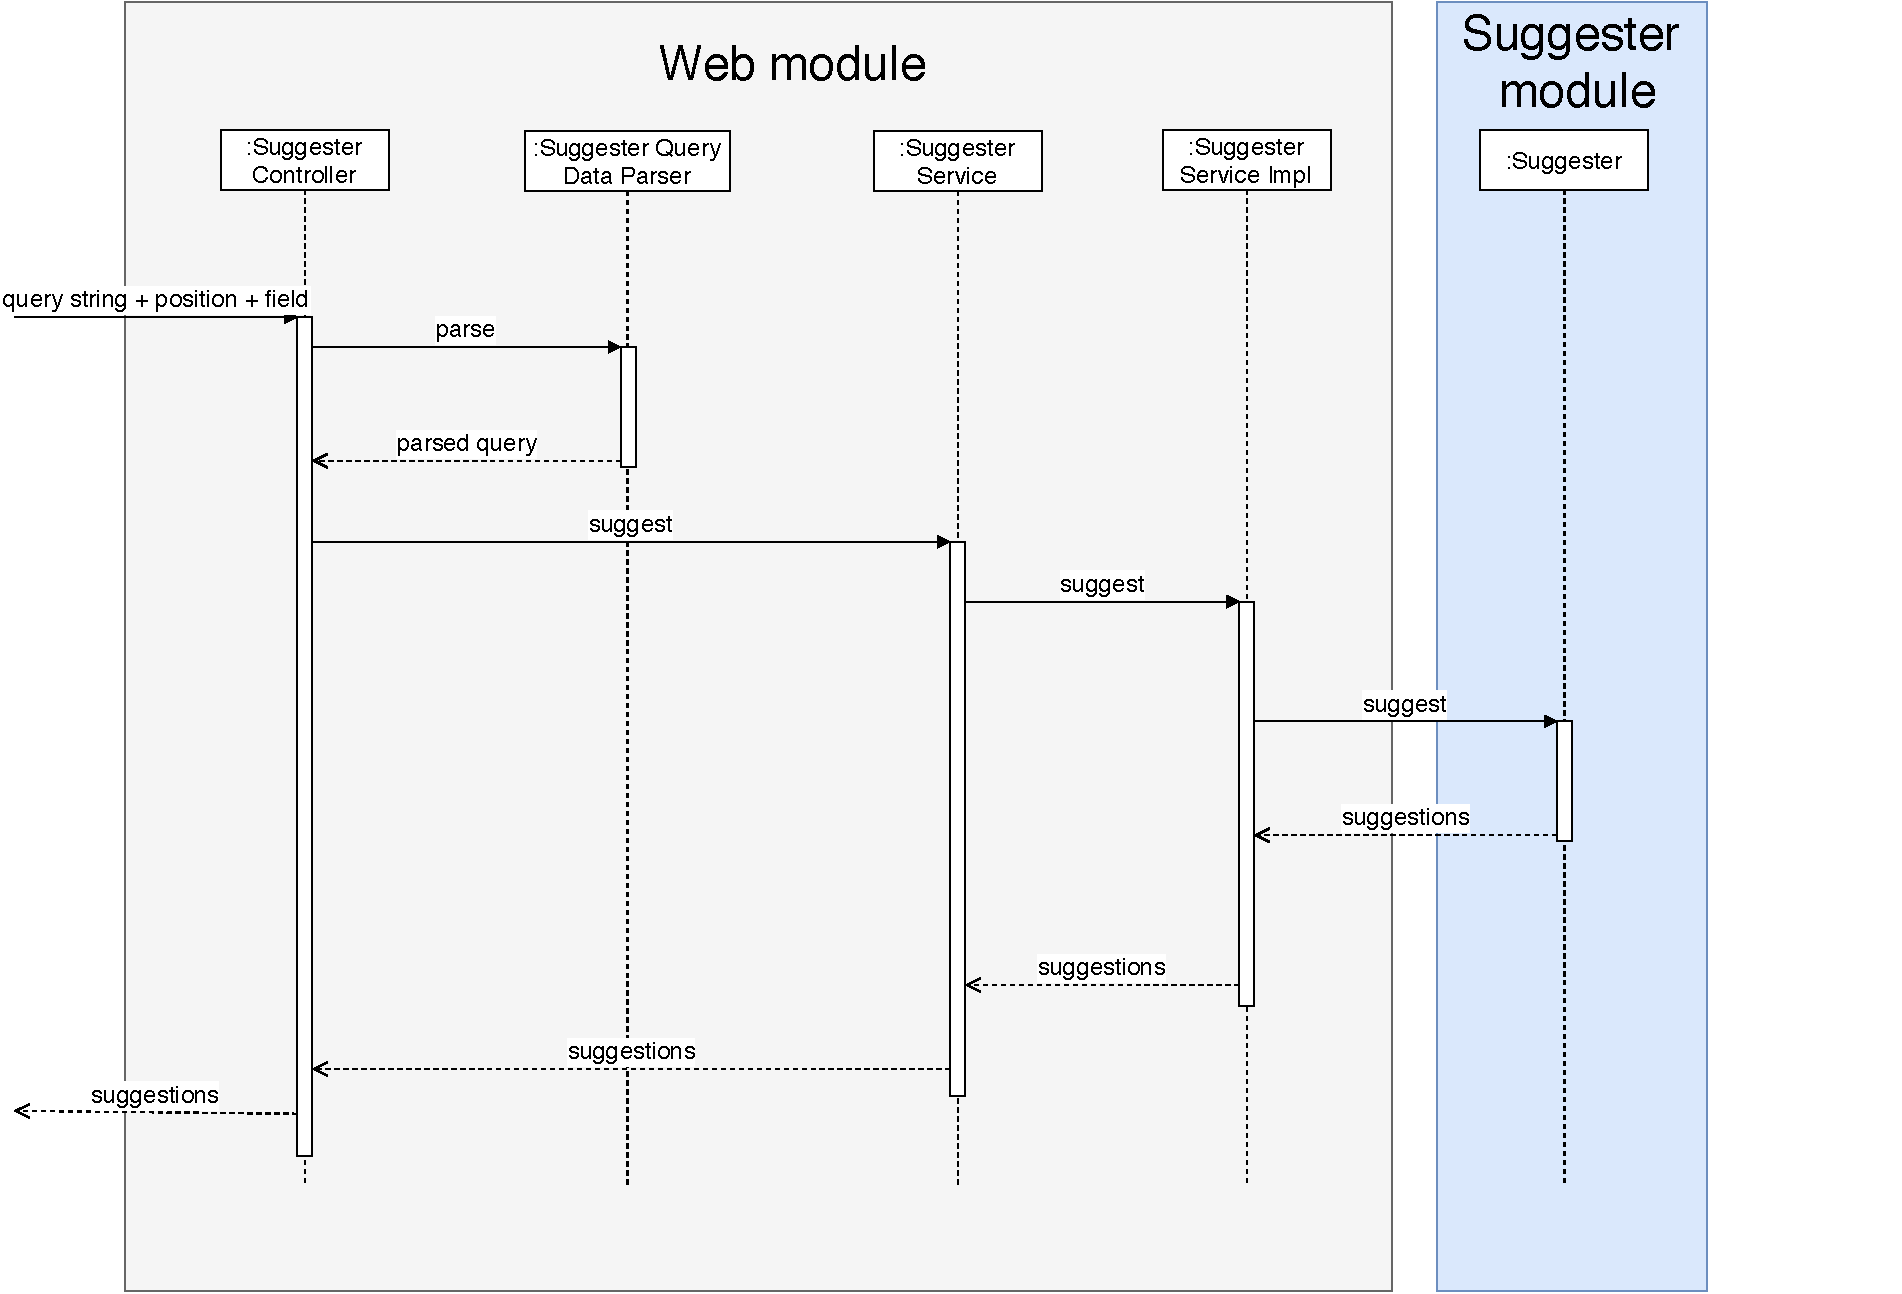
\includegraphics[width=145mm]{../img/programmer_sequence.pdf}
    \caption{Overview of the main object interactions}
    \label{programmer_sequence}
\end{figure}

\section{Web module}

\subsection{Suggester app}

\section{Suggester module}

\subsubsection{Public API}

\subsubsection{Detecting index version}

\subsubsection{Configuration change}

\subsubsection{Data structures abstractions}
